%\documentclass[handout]{beamer} % set [handout] as an option to remove /pause breaks
\documentclass{beamer}
\usetheme{McMaster}
\beamertemplatenavigationsymbolsempty 
\usepackage{tikz}
\usepackage[export]{adjustbox} % for left/right justifying images
\title{Teaching a Dog to Catalog: An Abbreviated History of Large Language Models and an Inquiry as to Whether They Can Replace Us}
\author{John Fink}
\institute{McMaster University}
\date{October 24, 2023}

% Talk is 2023-10-24 11am, Halifax, Access Conf
% History (briefer than may's talk)
% Ethical Considerations (maybe put them front and centre, like:
% 	I don't address:
%	Copyright/ethics
%	Pedagogy/academic honesty 
% Difference between *tuning*(including LoRA) and *vector*/document retrieval
% Important LLM (including ChatGPT concepts)
%	context size
%	parameters (7b, 13b, 30b, 65b)
%	Training (Lora, RLHF, few-shot, zero-shot) 
%	Temperature and those other llama.cpp variables (which I think are
%	common to all LLMs)
%	The Prompt
% Other proprietary LLMs (slightly less exasperated sigh)
%	Bard? Anthropic? BERT/RoBERTa?
% Open Source LLMs
% 	Meta's LLaMa
% 	LlaMa Leak
%	Hugging Face
%	Everything else!!!!
%	Non-LLaMa models
% 		StarCoder, RedPajama, etc. etc. etc.
%	Two ways to run local
%		CPU vs GPU
% 		emphasize that CPU is *many factors slower* than GPU
% The Future is Small:
% 	Environmental/other impact of Big Giant Systems
%		Water, electricity, etc
% Altering models:
% 	What is training? 
%	What is fine-tuning?
%	What is ... retreival (RAG? other? find out)
\begin{document}
\begin{frame}
    \maketitle
\end{frame}

\begin{frame}
	John Fink
	
	Digital Scholarship Librarian
	
	McMaster University
\end{frame}

% LAND ACQ HERE: 
% 

% McMaster University stands on the traditional territory shared between the Haudenosaunee  confederacy and the Anishinabe nations. This territory is covered by the Upper Canada Treaties, is within the lands protected by the “Dish With One Spoon” wampum agreement and is directly adjacent to Haldiman Treaty territory.

% We must acknowledge a debt to those who were here before us, and recognize our responsibility, as guests, to respect and honour the intimate relationship Indigenous peoples have to this land. 


\begin{frame}
	A (series of) disclaimers:
\end{frame}
 
 % Disclaimers: procrastination (for a reason), English major, many many demos, and randomness in those demos. No idea what's going to be said or anything. Will address ChatGPT but it is not at all the point of the talk generally.
 % ASK ME QUESTIONS ANYTIME. I don't know if this will take 30 minutes, 1 hour, 1.5 hours. Things may break. Things might crash. I could use the distraction.

 \begin{frame}[plain]
 	\makebox[\linewidth]{
\includegraphics[width=\paperwidth,height=\paperheight]{dontknow}}
 \end{frame}

 \begin{frame}
 	What is \textit{randomness}?
 \end{frame}

\begin{frame}[c]
	\centering
	\Huge
	Yijing / I-Ching
	
	(1000-750 BC)
\end{frame}
  
  % Wikipedia: as a divination text, the I Ching is used for a traditional Chinese form of cleromancy known as I Ching divination, in which bundles of yarrow stalks are manipulated to produce sets of six apparently random numbers. Each of the 64 possible sets corresponds to a hexagram, which can be looked up in the I Ching. The hexagrams are arranged in an order known as the King Wen sequence. The interpretation of the readings found in the I Ching has been endlessly discussed and debated over the centuries. Many commentators have used the book symbolically, often to provide guidance for moral decision-making, as informed by Confucianism, Taoism and Buddhism. 
  
  \begin{frame}[plain]
  	\makebox[\linewidth]{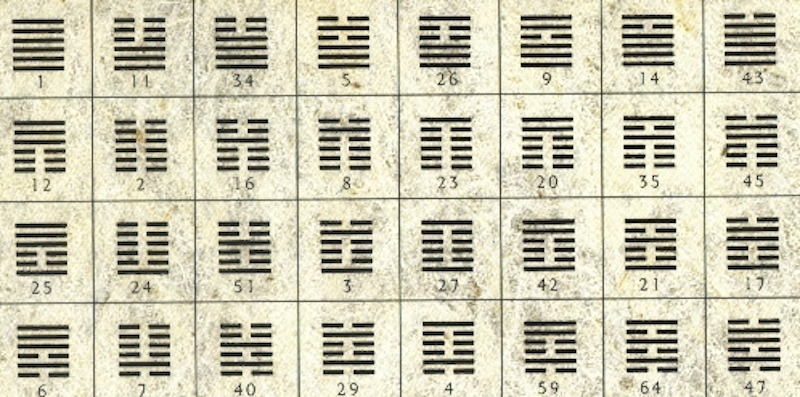
\includegraphics[width=\paperwidth,height=\paperheight]{i-ching.jpg}}
  \end{frame}
  \begin{frame}[c]
  	\centering
  	\Huge
  	The Man in the High Castle
  	
  	(1962)
  \end{frame}

% Wiki: Throughout the story, the characters make important decisions based upon their interpretations of prophetic messages from the I Ching, a Chinese book of divination.

\begin{frame}[plain]
	\makebox[\linewidth]{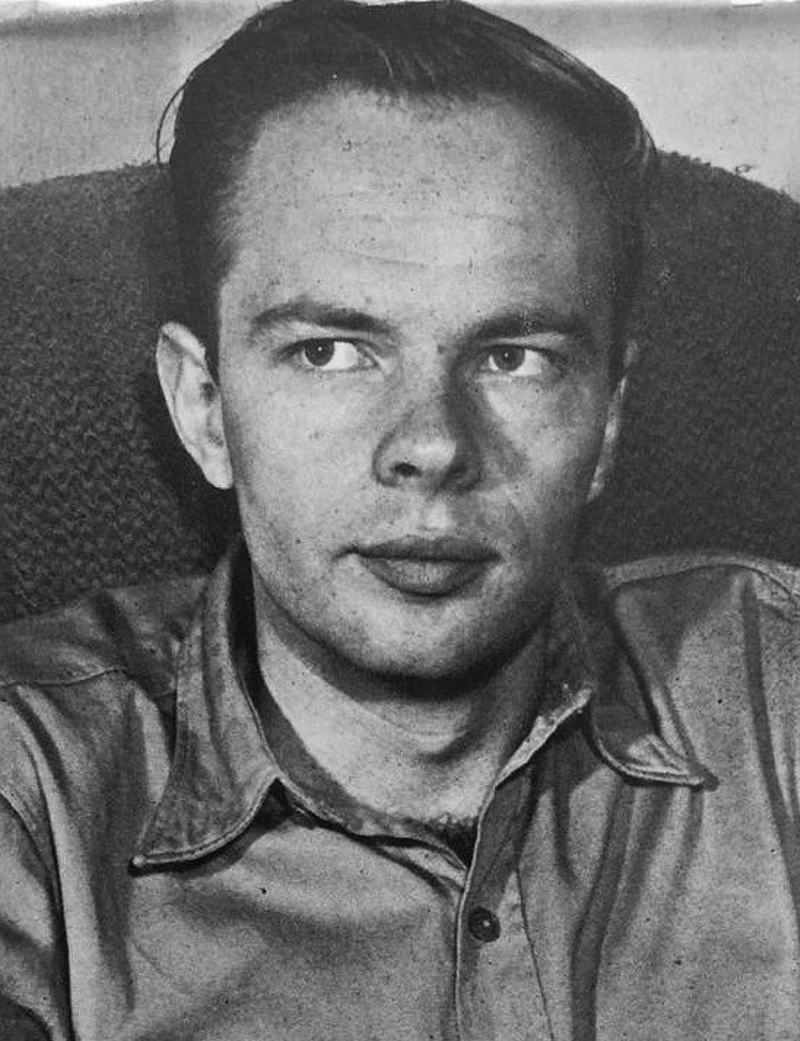
\includegraphics[height=\paperheight]{pkd.jpg}}
\end{frame}

% As a novelist, Dick used the I Ching to craft the themes, plot and story of The Man in the High Castle, whose characters also use the I Ching to inform and guide their decisions.

\begin{frame}[c]
	\centering
	\Huge
	Bibliomancy
	
	(1753 - as a term)
\end{frame}

\begin{frame}[plain]
	\makebox[\linewidth]{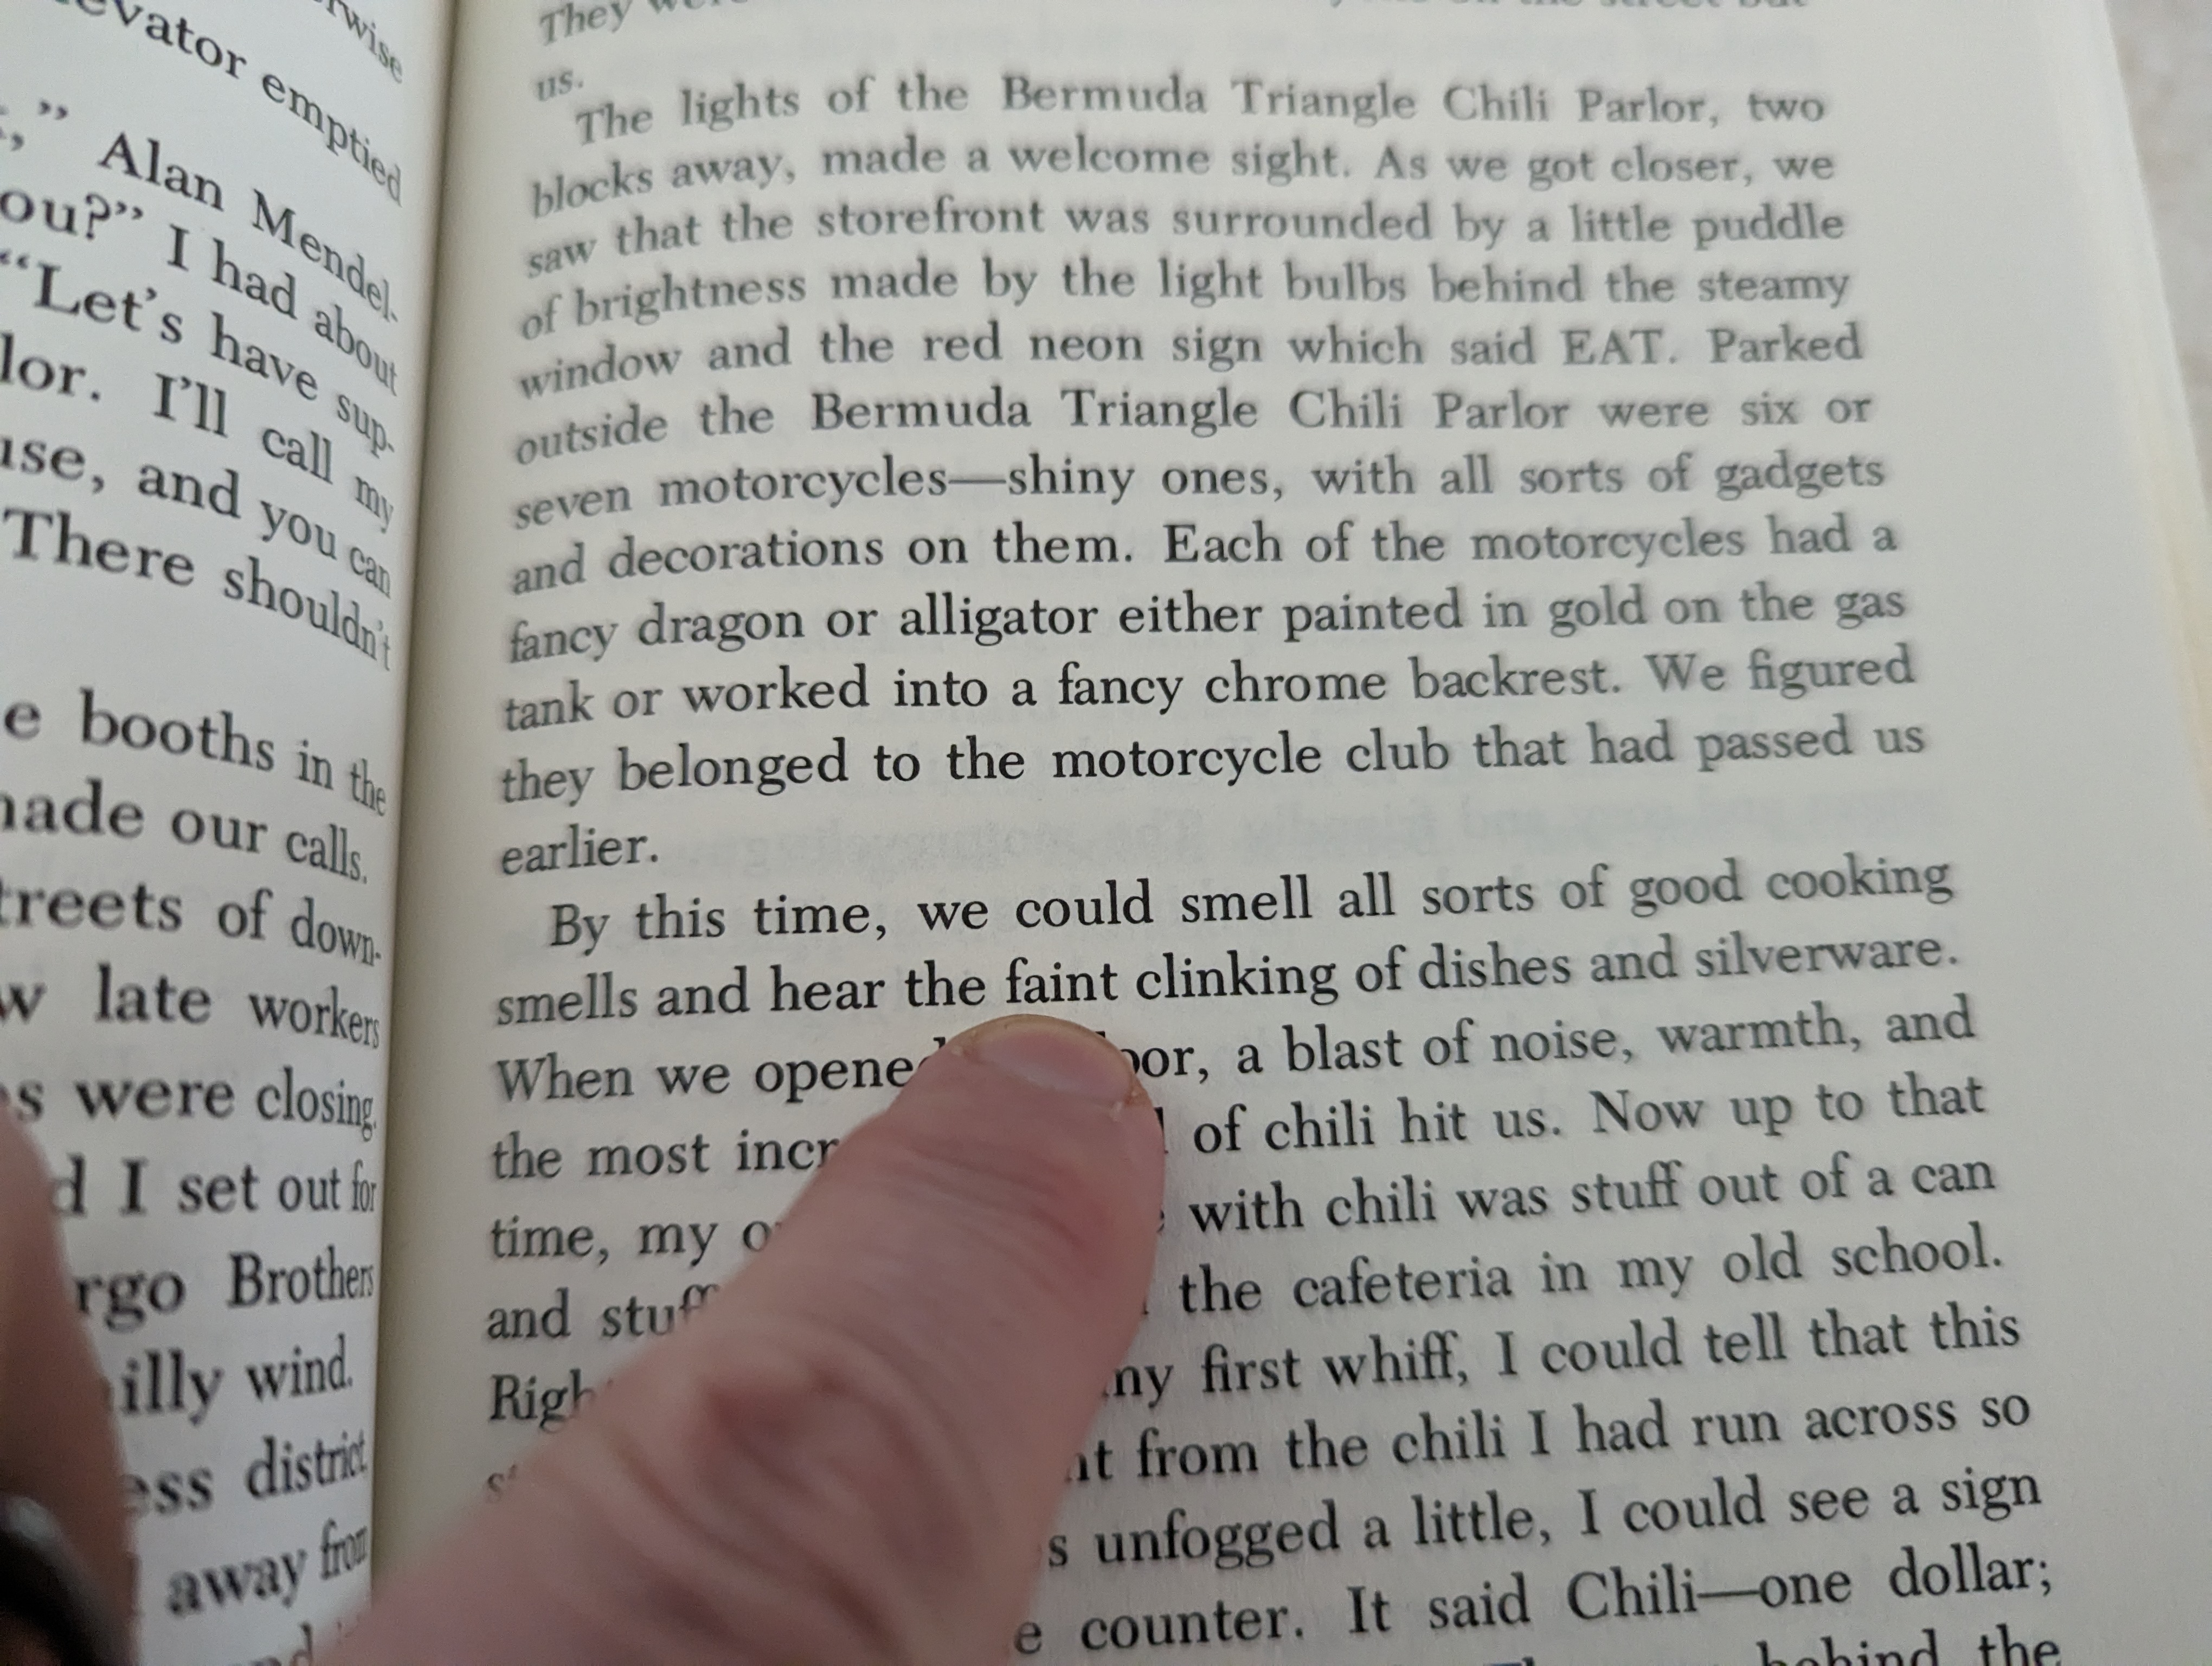
\includegraphics[width=\paperwidth,height=\paperheight]{pinkwater-bibliomancy.jpg}}
\end{frame}

%		A book is picked that is believed to hold truth.
%		It is balanced on its spine and allowed to fall open.
%		A passage is picked, with the eyes closed.
%		Usually done with a religious book.

\begin{frame}[c]
	\centering
	\Huge
	The Cut-Up Technique
	
	(1920s)
\end{frame}


\begin{frame}[plain]
	\makebox[\linewidth]{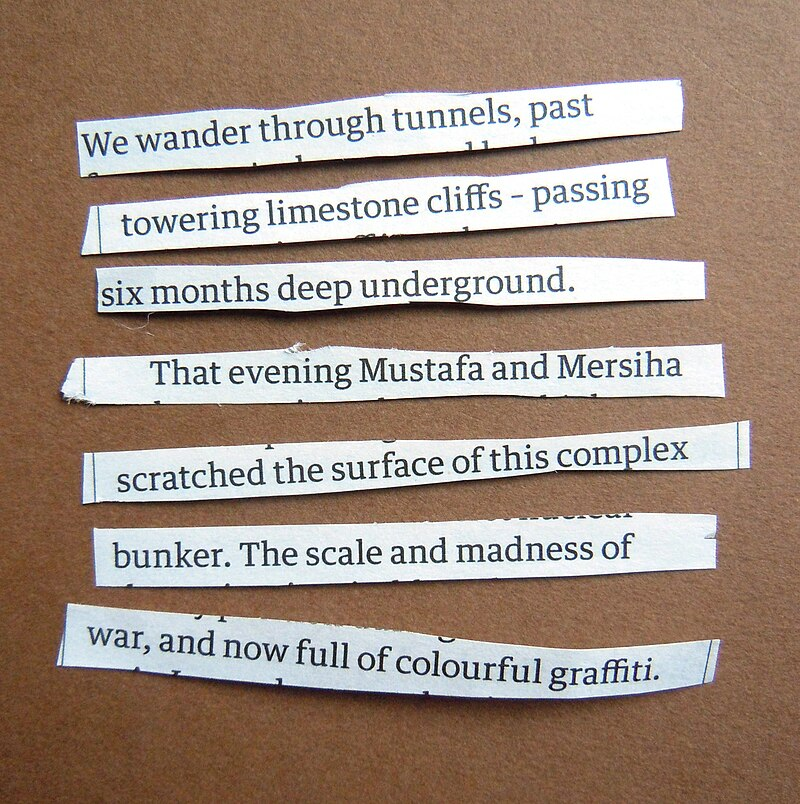
\includegraphics[width=\paperwidth,height=\paperheight]{cut-up.jpg}}
\end{frame}

% Started by the Dadaists in the 1920s but reached more exposure in the 1950s and 1960s with Canadian poet Brion Gysin and William S. Burroughs. 

\begin{frame}[c]
	\centering
	\Huge
	ELIZA
	
	(1966)
\end{frame}

\begin{frame}[plain]
	\makebox[\linewidth]{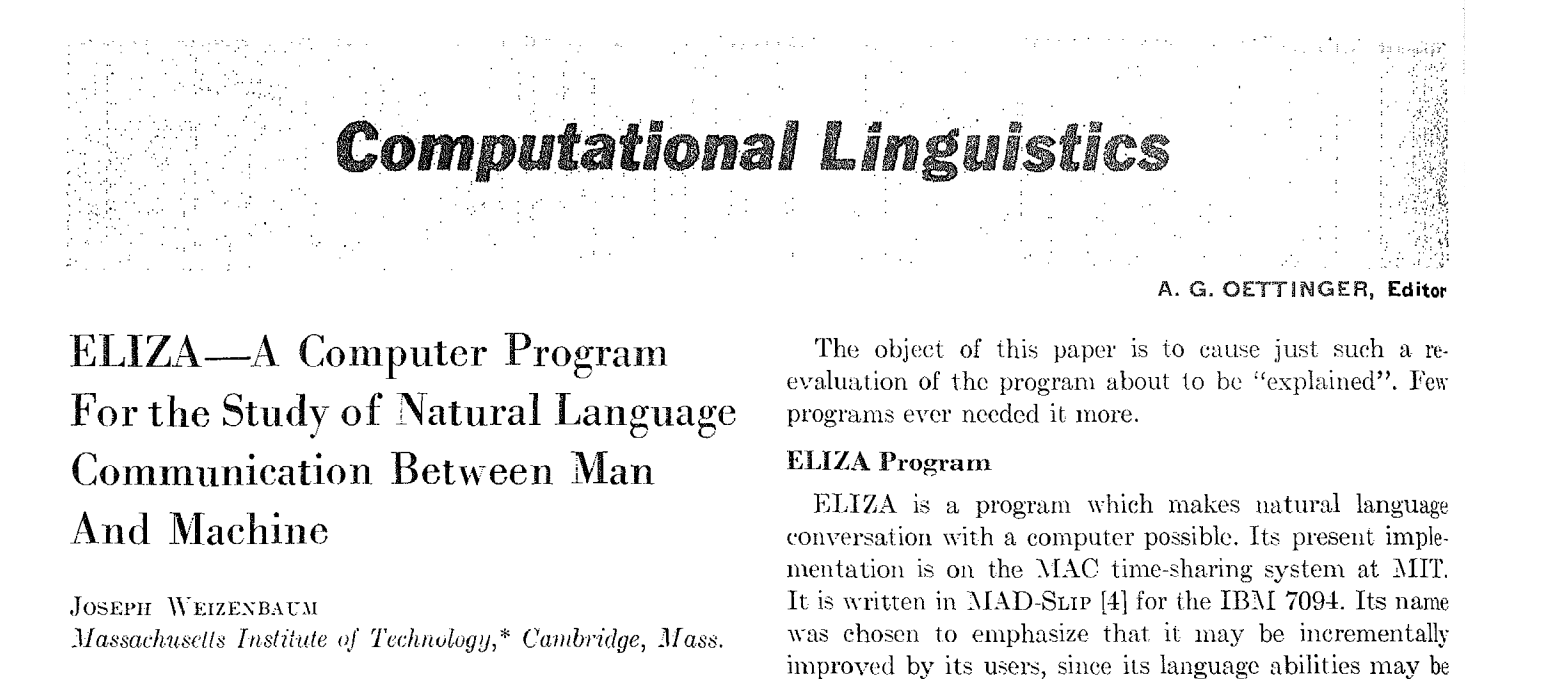
\includegraphics[width=\paperwidth,height=\paperheight]{eliza-paper}}
\end{frame}

% early natural language processing computer program created from 1964 to 1966[1] at MIT by Joseph Weizenbaum. Uses a pattern matching and subtitution methodology that really blew people's minds in 1966 -- many people were really convinced that Eliza had intelligence and understanding.

\begin{frame}[c]
	\centering
	\Huge
	Oblique Strategies
	
	(1975)
\end{frame}

% Made by Brian Eno and Peter Schmidt in 1975. Designed to help people with creativity and overcoming mental blocks in creative endeavours. Each card contains a gnomic suggestion that is supposed to break through those blocks.

\begin{frame}[plain]
	\makebox[\linewidth]{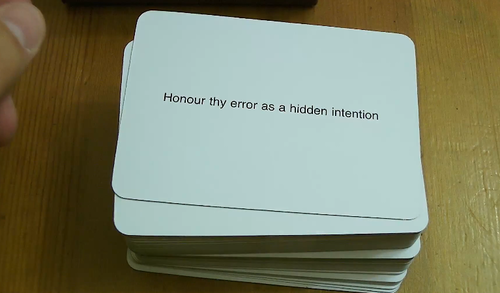
\includegraphics[width=\paperwidth,height=\paperheight]{oblique}}
\end{frame}

\begin{frame}[c]
	\centering
	\Huge
	Rogue
	
	(1980)
\end{frame}

% Rogue was originally developed around 1980 for Unix-based minicomputer systems as a freely distributed executable. It was later included in the Berkeley Software Distribution 4.2 operating system (4.2BSD).
% no game is the same as any previous one, as the dungeon levels, monster encounters, and treasures are procedurally generated for each playthrough. Origin of the term "Roguelike", now a massive genre of games in its own right.

\begin{frame}[plain]
	\makebox[\linewidth]{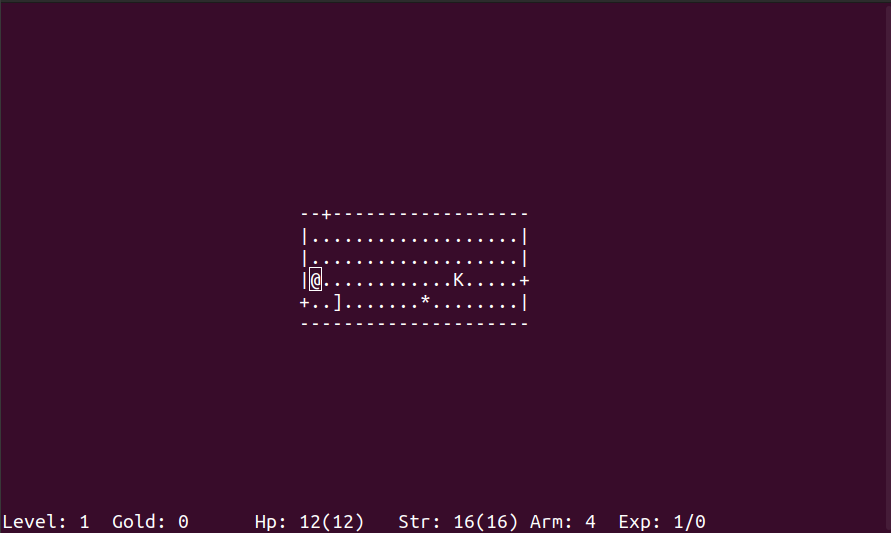
\includegraphics[width=\paperwidth,height=\paperheight]{rogue}}
\end{frame}

\begin{frame}[c]
	\centering
	\Huge
	Murder on the Zinderneuf
	
	(1983)
\end{frame}

\begin{frame}[plain]
	\makebox[\linewidth]{
\includegraphics[width=\paperwidth,height=\paperheight]{zinderneuf}}
\end{frame}

\begin{frame}[plain]
	\makebox[\linewidth]{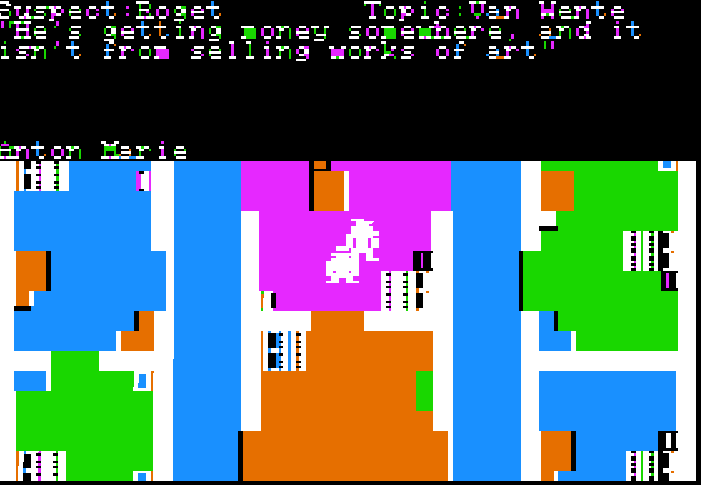
\includegraphics[width=\paperwidth,height=\paperheight]{zinderneuf2}}
\end{frame}

% Early attempt at random narrative play. wiki: "The game is set in 1936. The player is a detective traveling across the Atlantic aboard the world's most luxurious dirigible, the Zinderneuf. The craft is full of high-profile personalities from all walks of life. A murder takes place aboard the Zinderneuf, and it is up to the player to identify the culprit before the ship lands.", "The player is presented with a different murderer and victim each time the game is played. This, combined with the depth of narrative detail in the stories and characters, makes the game highly replayable. Each real-time game finishes in 36 minutes to encourage many replays."

\begin{frame}[c]
	\centering
	\Huge
	Racter and The Policeman's Beard
	
	(1984)
\end{frame}

\begin{frame}[plain]
	\makebox[\linewidth]{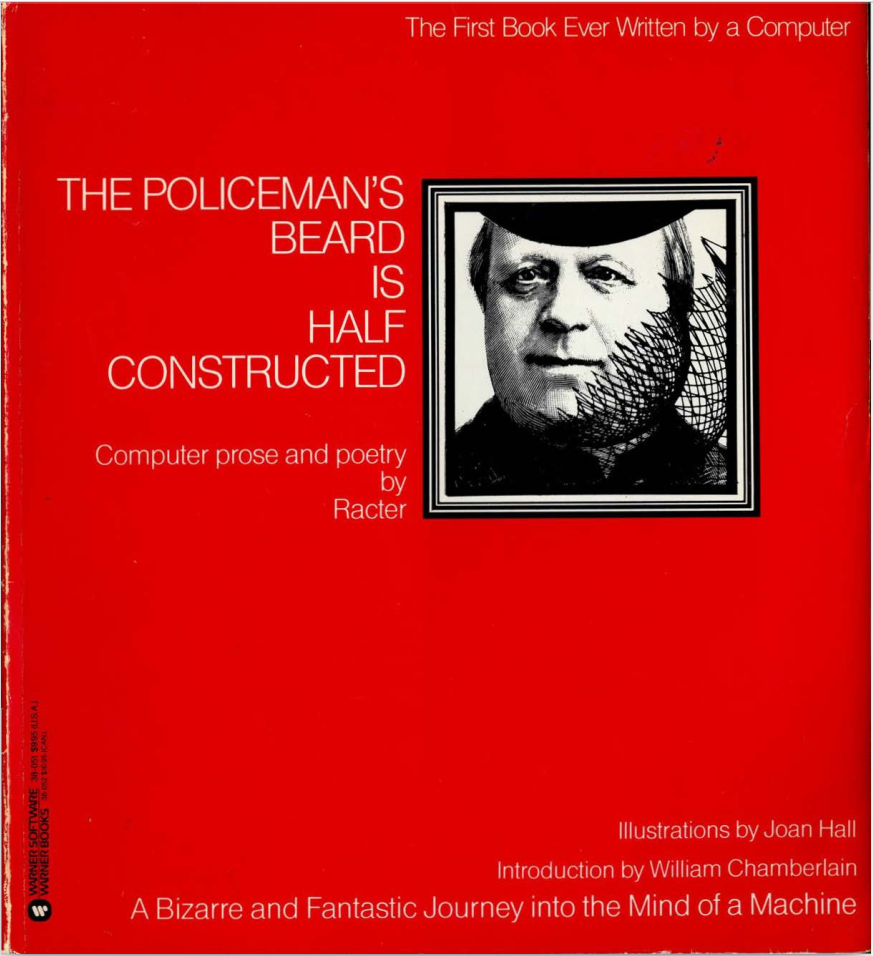
\includegraphics[height=\paperheight]{policemans-beard}}
\end{frame}

\begin{frame}[plain]
	\makebox[\linewidth]{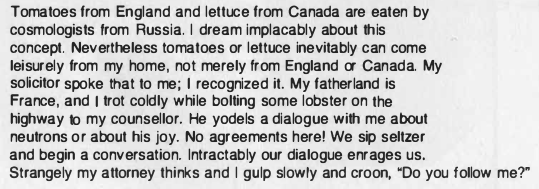
\includegraphics[width=\paperwidth,height=\paperheight]{beard-sample}}
\end{frame}

% Two versions of this program -- one for the book, purported to be extremely (uh, for the time) sophisticated (probably not, though) and one released commercially in 1984. Wiki: "However, in 1984 Mindscape released an interactive version of Racter, developed by Inrac Corporation, for IBM PC compatibles, Amiga, and Apple II computers. The published Racter was similar to a chatterbot. The BASIC program that was released by Mindscape was far less sophisticated than anything that could have written the fairly sophisticated prose of The Policeman's Beard. The commercial version of Racter could be likened to a computerized version of Mad Libs, the game in which you fill in the blanks in advance and then plug them into a text template to produce a surrealistic tale."

% racter demo here -- run in Chrome: run https://archive.org/details/msdos_Racter_1984


\begin{frame}{so, to recap:}
	\begin{itemize}
		\item 1000BC - Yijing / I-Ching
		\pause
		\item 1000BC-2017AD - some inconsequential stuff happens
	\end{itemize}
\end{frame}

\begin{frame}[c]
	but wait!
	
	\centering
	\Huge
	Danny Dunn and the Homework Machine
	
	(1958)
\end{frame}

\begin{frame}[plain]
	\makebox[\linewidth]{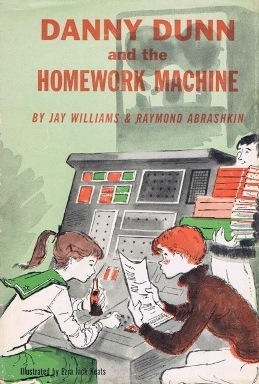
\includegraphics[height=\paperheight]{dannydunn.jpg}}
\end{frame}

% Very interesting, this. Danny Dunn is a series of books about a young precocious kid with vaguely scientific themes -- there's one about anti-gravity paint, one about home automation, one about controlling the weather. The Homework Machine book opens with Danny Dunn working on a device -- the polygraph -- that connects one pen to another pen, so that when the first pen writes the second pen duplicates that writing, so that Danny Dunn's buddy can do, say, their English homework and Danny can do math, or whatever. But Danny wants to have a machine do his homework for him autonomously -- sound familiar? -- and the professor he lives with has just such a machine, which is programme%The 1958 / Danny Dunn thing should probably go right before you actually talk about LLMsd by English prompts. Danny and his gang are getting a lot of homework, so they feed it into the machine and it does their homework for them. They eventually get caught and learn Valuable Lessons, and it's pointed out that in *training* the machine they may have done more homework than the actual homework.

\begin{frame}
	A little conversation about the weather.
\end{frame}

\begin{frame}[plain]
	\makebox[\linewidth]{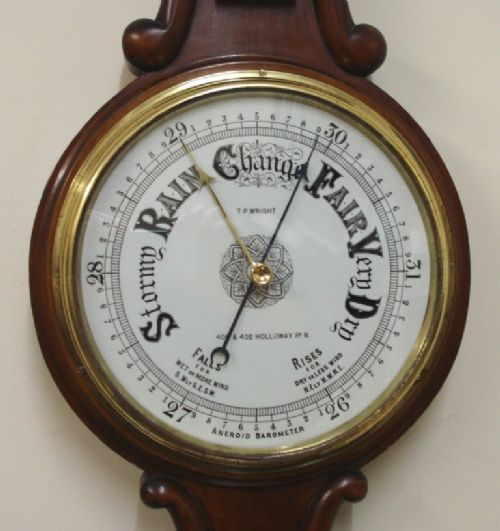
\includegraphics[width=\paperwidth,height=\paperheight]{barometer}}
\end{frame}

\begin{frame}[plain]
	\makebox[\linewidth]{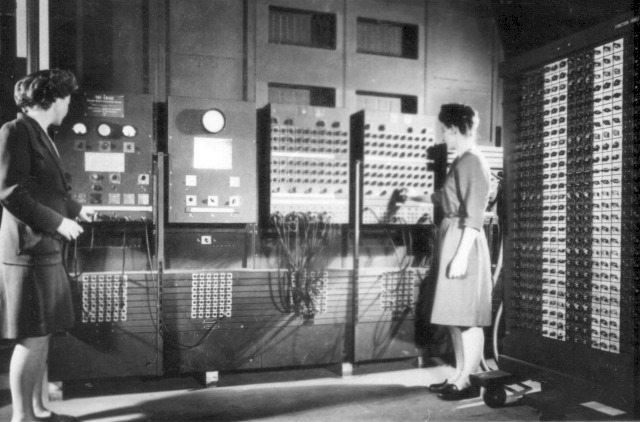
\includegraphics[width=\paperwidth,height=\paperheight]{eniac}}
\end{frame}

% Weather prediction is a lot like language prediction in LLMs. Before the advent of programmable computers, it involved looking at the sky a lot and looking at barometers a lot -- in the 1950s, the early computer ENIAC ran some of the first weather models. Nowadays, we have weather models that are extremely sophisticated and take a lot of computing power to run and can predict the weather many days out. They predict the weather by looking at *current conditions* and extrapolating what *usually happens* from those current predictions, and they're really pretty good at it because there's a lot of data about. This is *eerily similar* to how LLMs/ChatGPT works -- it's not "reasoning" per se, but *predicting* what comes next based on context and what has come previous, and since they have vast, vast amounts of example data -- like the weather models! -- they are pretty good at it. Good enough to fool us, anyway.

\begin{frame}
	Why I say "Large Language Model" and not "AI"
\end{frame}

% I tend to be pretty sure that the term "AI" is not useful here, not because it's true or not true, but because it's *unknowable*, at least by current definitions of "Intelligence". 

% Talking dog parable: “TALKING DOG FOR SALE.” The owner took him to the
%backyard and left him with an old Border Collie. The dog looked up and said:
%“Woof. Woof. Hi, I’m Carl, pleased to meet you.”
%The driver was stunned. “Where did you learn how to talk?”
%“Language school,” said Carl, “I was in a top secret language program with the CIA.
%They taught me three languages:
%How can I help you? как я могу вам помочь? 我怎么帮你?”
%“That’s incredible,” said the driver, “What was your job with the CIA?”

%“I was a field operative and the CIA flew me around the world. I sat in a corner and
%eavesdropped on conversations between foreign agents and diplomats, who never suspected I
%could understand what they were saying, and reported back to the CIA what I overheard.
%“You were a spy for the CIA?” said the driver, increasingly astonished.
%“When I retired, I received the Distinguished Intelligence Cross, the highest honor awarded by
%the CIA, and honorary citizenship for extraordinary services rendered to my country.”
%The driver was a little shaken by this encounter and asked the owner how much he %wanted for
%the dog.
%“You can have the dog for $10.”
%“I can’t believe you are asking so little for such an amazing dog.”
%“Did you really believe all that bullshit about the CIA? Carl never left the farm.


% SPECIAL CODE WORD HERE: HAL


\begin{frame}
	So, about 2017...
\end{frame}

\begin{frame}[plain]
	\makebox[\linewidth]{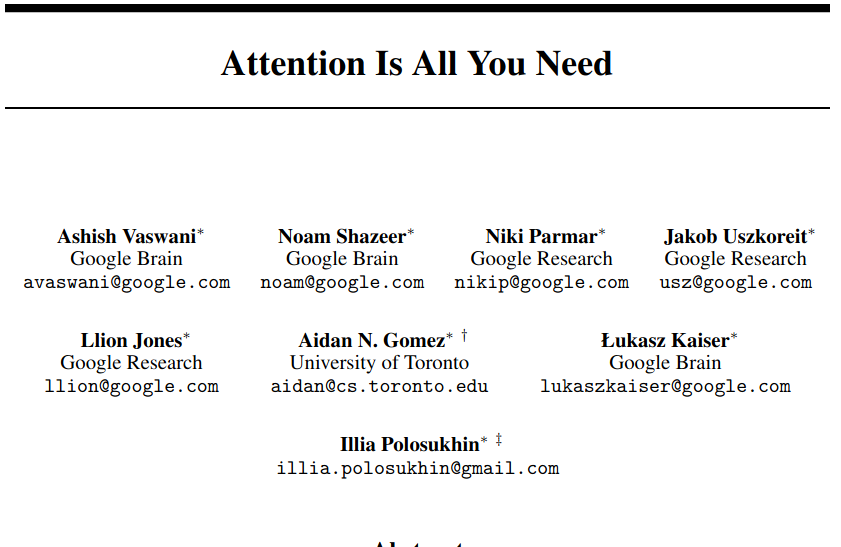
\includegraphics[width=\paperwidth,height=\paperheight]{attention}}
\end{frame}

% this is the big one. This is what kick-started *everything* we see today. Prior to this, language generators were goofy and easy to spot as being goofy -- think Racter, think Eliza, think Markov chaining. Not going to fool anyone. After this, pow, the gates are busted open. ChatGPT comes out of this, as well as almost every other recent generative AI that you know of. An absolutely fundamental paper that I *cannot understand*.

\begin{frame}{2017-now! Right now!}
	\begin{itemize}
		\item 2017 - "Attention Is All You Need" paper
		\pause
		\item 2018 - "Improving Language Understanding by Generative Pre-Training" paper
		\pause 
		\item 2020 - "Language Models are Few-Shot Learners" paper (GPT-3)
		\pause
		\item 2022 - InstructGPT, and then ChatGPT
		\pause
		\item 2023 - and then....
	\end{itemize}
\end{frame}

\begin{frame}[plain]
	\makebox[\linewidth]{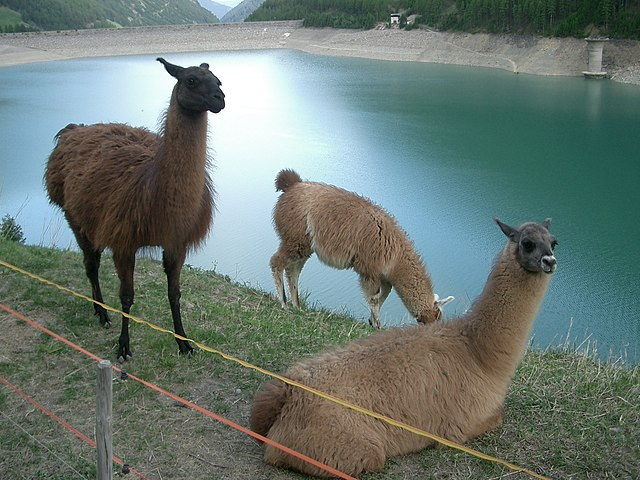
\includegraphics[width=\paperwidth,height=\paperheight]{llamas}}
\end{frame}

% February 24th, Facebook introduces LLaMa in a blog post but doesn't freely release how it's made, but it *does* let people have access to it via an application. Of course it was *instantly* leaked, and started an absolute torrent of derivatives. Nearly every locally-runnable model today is based somewhat on the LLaMa original code, which is problematic because it precludes commercial use. There are attempts -- going on RIGHT NOW -- to recreate LLaMa functionality with unencumbered data, and there are already models out there without encumbrances, so this is less of a factor going forward.

\begin{frame}
	"Progress is now moving so swiftly that every few weeks the state-of-the-art is changing or models that previously required clusters to run now run on Raspberry PIs."
	 
	 -- https://github.com/brexhq/prompt-engineering
\end{frame}

% Usually LLMs need to run on very beefy graphics cards with lots and lots of VRAM, especially during the training phase. But there are methods to run these models on way more modest hardware and only on the CPU and get decent performance -- of course, not nearly as fast as using GPUs but *very usable* and, more importantly, cheap, cheap, cheap. The raspberry pi in question costs around $100CAD, and *just the graphics card* for a capable GPU-based setup will run about $6000.

\begin{frame}{Important concepts for GPT and other models}
	\begin{itemize}
		\item Context Window and Tokens
		% 2k for LLaMa, 4k for GPT4 chat, 8k/32k via API. This is short term memory.
		\pause
		\item Few-Shot / No-Shot
		\pause
		\item Parameters
		% GPT-1 117m, GPT-2 1.5b, GPT-3 175b, GPT-4 170t 
		\pause
		\item Training
		\pause 
		\item The Prompt, aka "Programming for English Majors"
		\pause
		\item And the Random Seed.
	\end{itemize}
\end{frame}

\begin{frame}
	\begin{itemize}
		\item Context Window is the "memory" of an LLM
		\pause
		\item And Tokens -- words, roughly -- fill up that "memory"
		\pause
		\item And the \textit{response} also takes tokens.
	\end{itemize}
\end{frame}

% demo https://platform.openai.com/tokenizer

\begin{frame}[plain]
	\makebox[\linewidth]{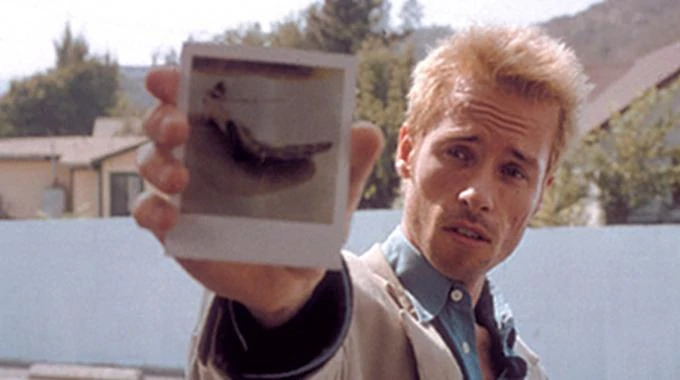
\includegraphics[width=\paperwidth,height=\paperheight]{leonard}}
\end{frame}

\begin{frame}{Few-Shot / No-Shot}
	\begin{itemize}
		\item \textit{Few-Shot} -- a few examples to "teach" an LLM, such as:
		\pause
		\item "I hate it when my phone battery dies." - negative
		\pause
		\item "My day has been great!" - positive
		\pause
		\item "Here is an article." - neutral
		\pause
		\item "This presentation is going fantastic!!!!" - positive(ly optimistic)
		\pause
		\item And \textit{No-Shot} is exactly what you think it is.
	\end{itemize}
\end{frame}

\begin{frame}{Training}
	\begin{itemize}
		\item Usually done on text corpuses
		\pause
		\item The Pile (825GiB), Github, ShareGPT, etc.
		\pause
		\item And other terms like RLHF (Reinforcement Learning from Human Feedback)
		\pause
		\item The larger the model, the more resources it takes to train or re-train.
	\end{itemize}
\end{frame}

\begin{frame}{Parameters}
	\begin{itemize}
		\item Roughly corresponds to how "Complex" or "Smart" a model is.
		\pause
		\item (...very roughly)
		\pause 
		\item But \textit{definitely} correlates to resources needed to run the model.
		\pause
		\item Which is why, say, GPT-4 requires this....
	\end{itemize}
\end{frame}



\begin{frame}[plain]
	\makebox[\linewidth]{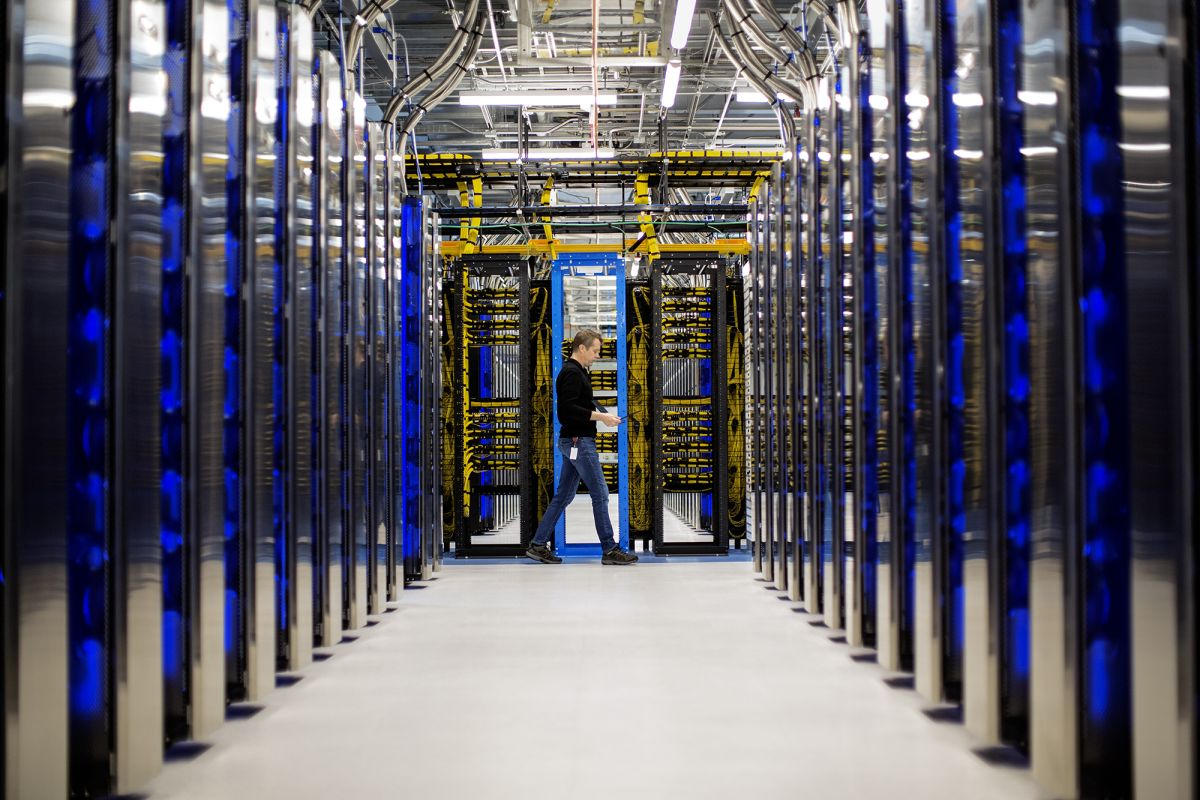
\includegraphics[width=\paperwidth,height=\paperheight]{azure-data-centre}}
\end{frame}

\begin{frame}
	And you can run a 7B model on this....
\end{frame}

\begin{frame}[plain]
	\makebox[\linewidth]{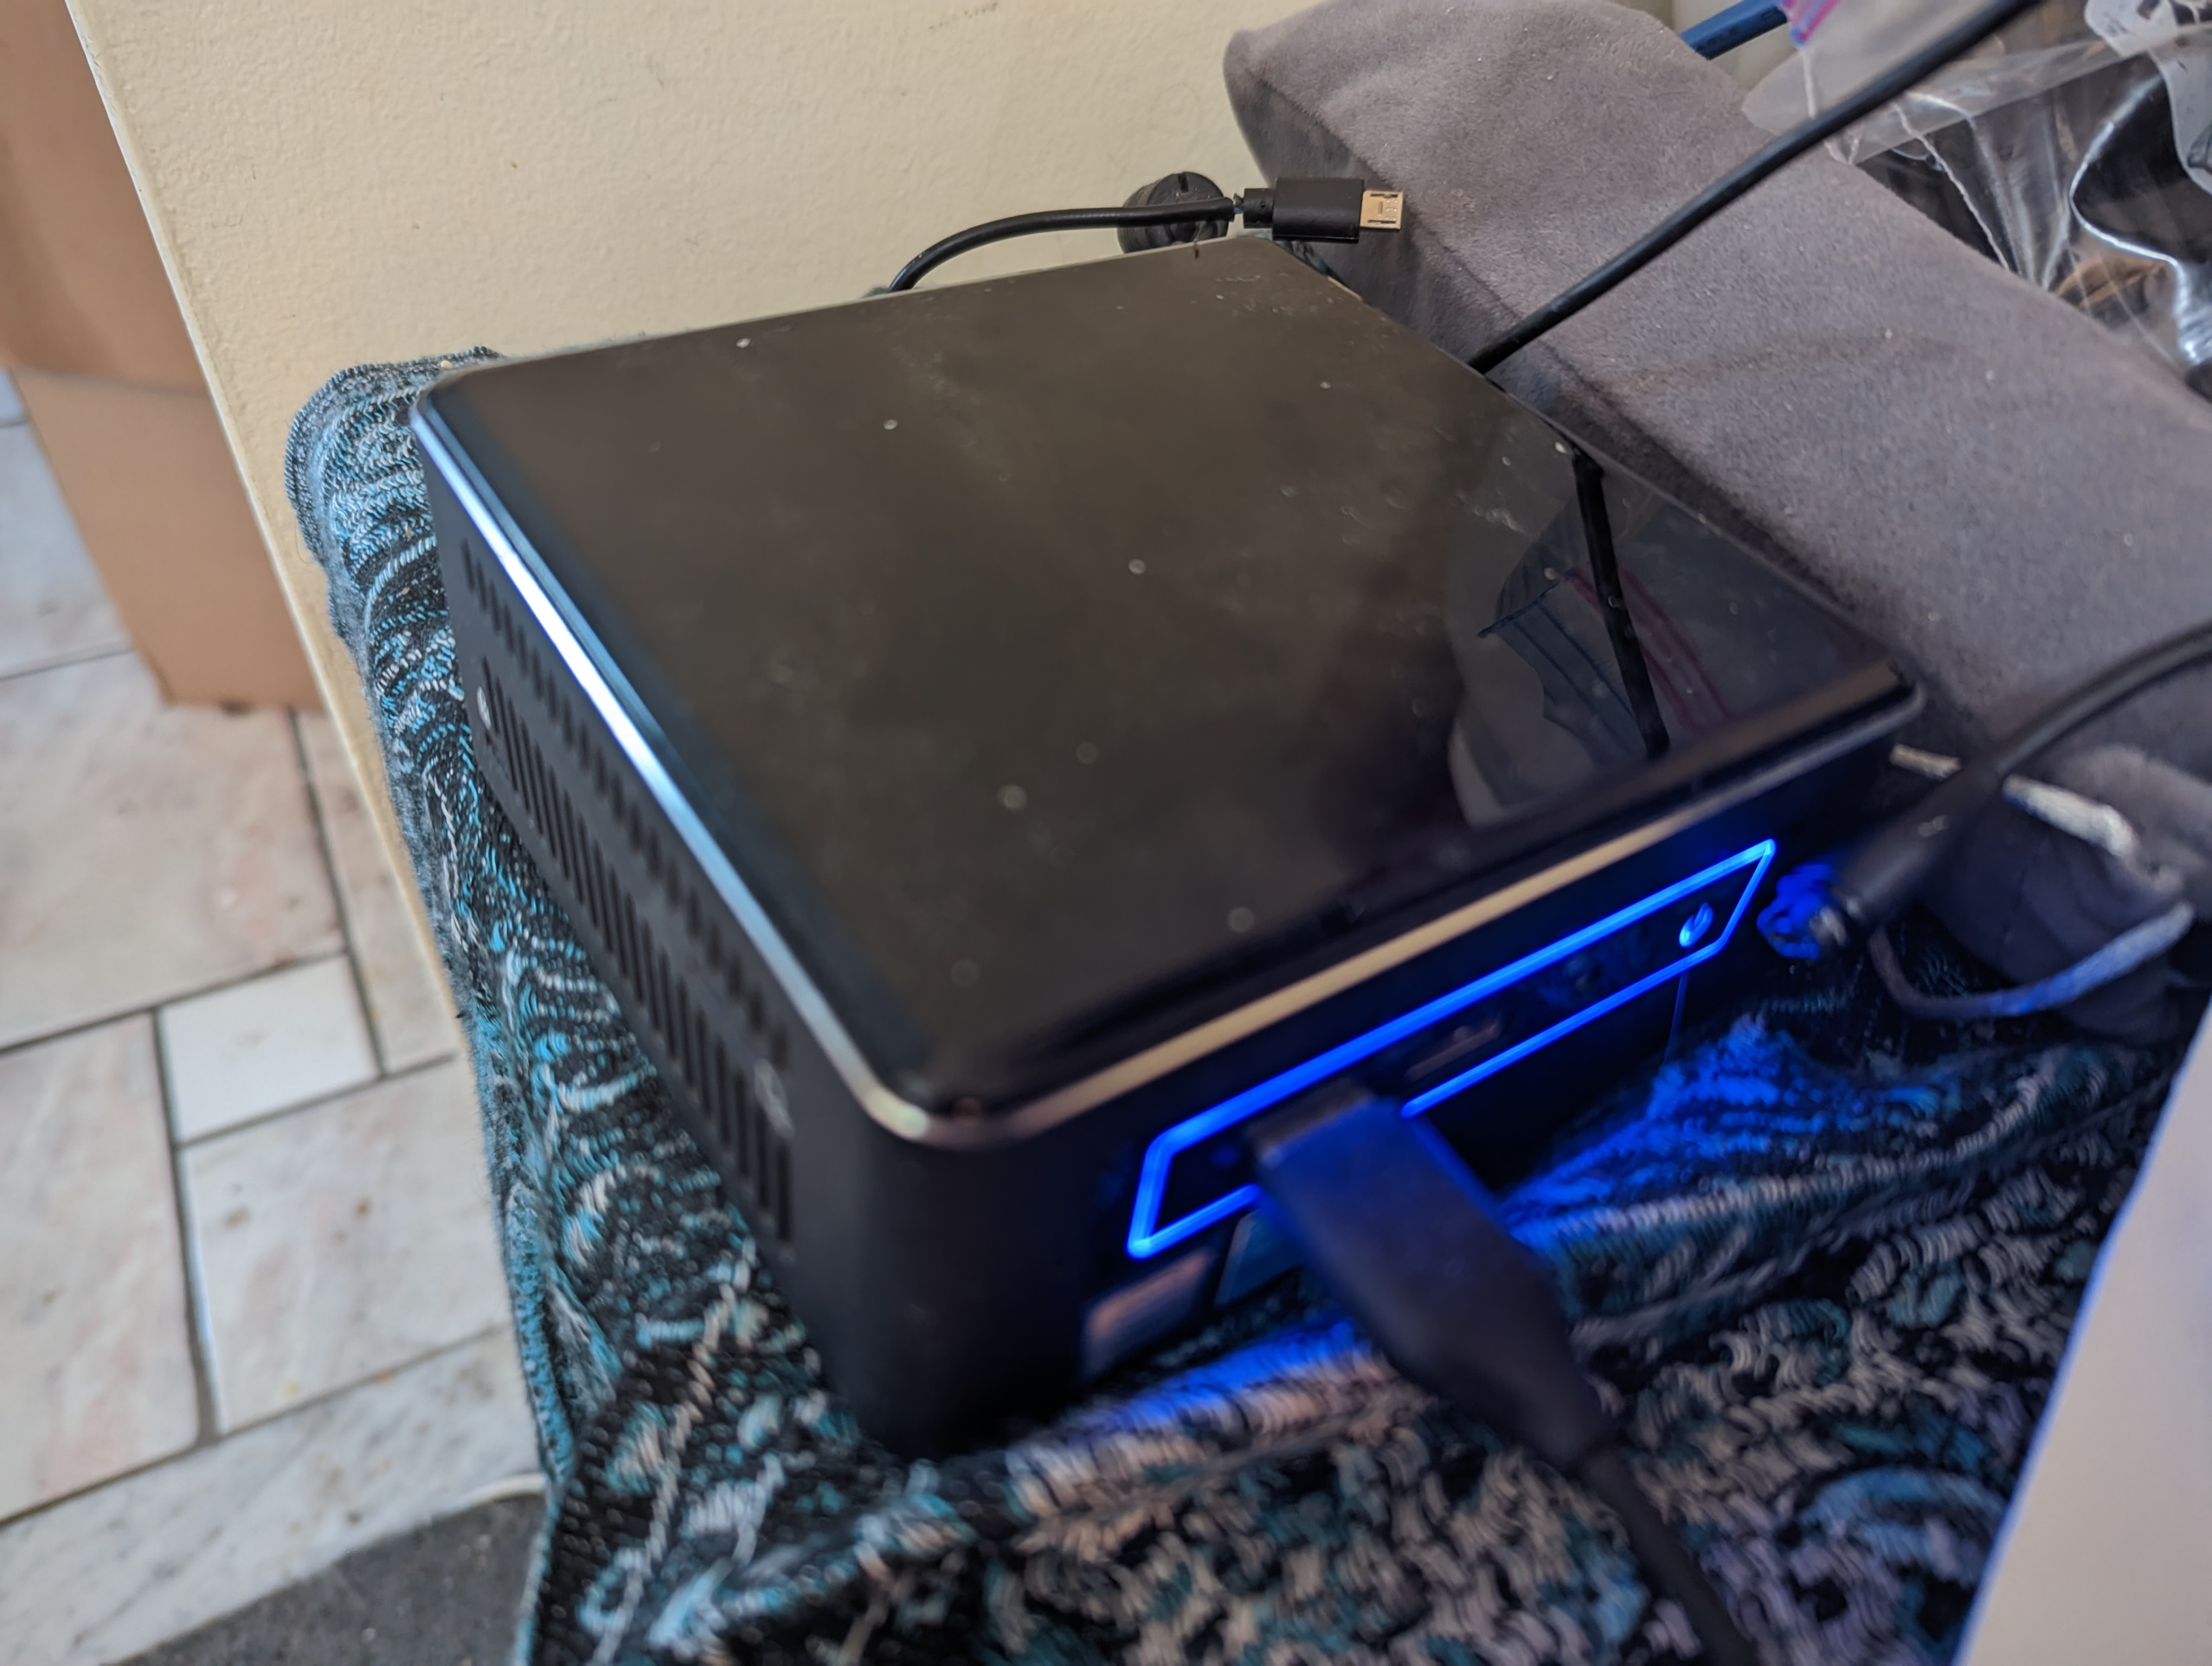
\includegraphics[width=\paperwidth,height=\paperheight]{pfeebe}}
\end{frame}


\begin{frame}
	llama.cpp -- https://github.com/ggerganov/llama.cpp
\end{frame}


% demo soup-to-nuts build of llama.cpp on pfeebe:
% git clone https://github.com/ggerganov/llama.cpp
% make clean; make LLAMA_OPENBLAS=1
% copy model file 
% Demo librarian.txt -- have it make up APA references for John Fink and then ask it the two apples / one banana logic problem
% Demo huggingface.co/chat
% also demo privateGPT if you have time.

% move this slide to *just* before you actually talk about LLMs.


\begin{frame}{We Have No Moat}
	In May (yes, the month that we are still in right now) a Google internal document was leaked to the public, titled "We Have No Moat, and Neither Does OpenAI". It's worth quoting some bits from it, because it's a doozy.
\end{frame}

\begin{frame}{We Have No Moat}
	\begin{itemize}
		\item "While our models still hold a slight edge in terms of quality, the gap is closing astonishingly quickly. Open-source models are faster, more customizable, more private, and pound-for-pound more capable. They are doing things with \$100 and 13B params that we struggle with at \$10M and 540B. And they are doing so in weeks, not months. This has profound implications for us."
		\pause
		\item "Indeed, in terms of engineer-hours, the pace of improvement from these models vastly outstrips what we can do with our largest variants, and the best are already largely indistinguishable from ChatGPT. Focusing on maintaining some of the largest models on the planet actually puts us at a disadvantage."
	\end{itemize}
\end{frame}

\begin{frame}{THE FUTURE OF LARGE LANGUAGE MODELS}
	\begin{itemize}
		\item ....Skynet????
		\pause
		\item ....fully automated luxury communism???
		\pause 
		\item ....larger context windows?
		
	\end{itemize}
	
	
	
\end{frame}

\begin{frame}
	%this is always the last slide
	Any questions?\\ 
	jfink@mcmaster.ca\\
	
\includegraphics[left, height=4mm]{mastodon} \hspace{1mm}  https://glammr.us/@jbfink
	
\end{frame}

\end{document}
